\chapter{Modification of TASC for Bending Models} \label{chap:tasc-development}

\section{Adding Bending Models to TASC Interpolation Database}
\label{sec:add_bending_models}

The 600 {.mat} files for bending models were created using the methods given in \Cref{sec:postprocess}, and need to be added to the 600 tension models in the TASC interpolation database described in \Cref{chap:app-verification-allen-wells}.
The tension models are stored in a four-dimensional array named \verb|result|, indexed by values of \(\frac{a}{t}\), \(\frac{a}{c}\), \(n\), and \(\frac{E}{\Sys}\), so the bending models will be stored in an identically-structured four-dimensional array named \verb|result_bending|.
\Crefrange{alg:create_bending_database}{alg:populate_structure_placeholders} show the procedure used to calculate values for the database, either by directly using results from the finite element models, or by applying mechanics of materials or basic fracture mechanics relations to find properties including the total load applied to a place or \Jel.

Noteworthy steps taken include converting the quarter-plate model reaction force to an equivalent reaction force, bending moment, and bending stress for a full plate under test, as the distance between the model's imaginary rollers varies as the plate deforms, unlike a physical test frame where the rollers would remain at a fixed distance:
\begin{align}
P_\text{model} &= -4(\text{WARP3D Reaction}) \\
M_\text{model} &= (P_\text{model})(\text{varying distance between rollers}) \\
P_\text{test} &= \frac{2 M_\text{model}}{\Souter-\Sinner} \\
M_\text{test} &= \frac{P_\text{test}}{2} \frac{\Souter-\Sinner}{2} \\
\sigma &= \frac{M_\text{test} t}{2 I}
\end{align}
and calculation of \Jel from \J, where it is assumed that for the first time step, \Jpl is zero, and that \Jel is proportional to the square of the applied load or applied moment:
\begin{align}
\Jel(\text{load step } i) &= \J(\text{load step 1}) \left(\frac{M(\text{load step } i)}{M(\text{load step 1})}\right)^2\quad.
\end{align}
Once the calculations are complete, values including \Jel, \J, CMOD, $\phi$, and reaction forces are written to the TASC interpolation database.

\begin{algorithm}[tbp]
  \caption{Create Bending Database}
  \label{alg:create_bending_database}
  \begin{algorithmic}
    \Procedure{Create Bending Database}{}
    \State (result, input) $\gets$ load values previously saved in interp\_solution\_database.mat
    \State result\_bending $\gets$ empty array of structures
    \State \(t, \nu)\) $\gets$ (1, 0.3) \Comment{plate thickness, Poisson's ratio}
    \State \(\frac{a}{t}\) Array $\gets$ $(0.2, 0.4, 0.6, 0.8)$
    \State \(\frac{a}{c}\) Array $\gets$ $(0.2, 0.4, 0.6, 0.8, 1.0)$
    \State \(n\) Array $\gets$ $(3, 4, 6, 10, 20)$
    \State \(E\) Array $\gets$ $(100, 200, 300, 500, 700, 1000)$
    \ForAll{\(i\) in $(1, 2, 3, 4)$}
      \ForAll{\(j\) in $(1, 2, 3, 4, 5)$}
        \State \(\frac{a}{t}\) $\gets$ index \(i\) of \(\frac{a}{t}\) Array
        \State \(\frac{a}{c}\) $\gets$ index \(j\) of \(\frac{a}{c}\) Array
        \State \((a, c, W, \Sinner, \Souter, I, L)\) $\gets$ \Call{Calculate Geometry}{$\frac{a}{c}, \frac{a}{t}, t$}
        \ForAll{\(k\) in $(1, 2, 3, 4, 5)$}
          \ForAll{\(l\) in $(1, 2, 3, 4, 5, 6)$}
            \State \(n\) $\gets$ index \(k\) of \(n\) Array
            \State \(E\) $\gets$ index \(l\) of \(E\) Array
            \State File Pattern $\gets$ 'path/bend\_ac\((\frac{a}{c})\)\_at\((\frac{a}{t})\)\_*\_E\((E)\)\_n\((n)\)\_wrp.mat'
            \State \Comment{File Pattern should only match one file}
            \State (BC Value, Filename, Stress-Strain Curve) $\gets$ values from .mat file
            \State (Moment Arm, Reaction) $\gets$ values from .mat file
            \State \((P, M, \sigma)\) $\gets$ \Call{Calculate Statics}{Reaction, Moment Arm, \Sinner, \Souter, $I$, $t$}
            \State (\J, CMOD, \(\phi\)) $\gets$ values from .mat file
            \State \Comment{\J is a table with values for every load step and $\phi$}
            \State \((N_\text{steps}, N_\text{crack nodes}, \Jel, \phi)\) $\gets$ \Call{Calculate EPFM}{$\J, M, \phi$}
            \State (Structure.a, Structure.c, Structure.width, Structure.B) $\gets$ \((a, c, W, t)\)
            \State (Structure.S\_inner, Structure.S\_outer, Structure.length) $\gets$ \((\Sinner, \Souter, L)\)
            \State (Structure.reac\_force, Structure.moment, Structure.S\_bend) $\gets$ $(P, M, \sigma)$
            \State (Structure.Jel\_EPFM, Structure.Jtotal\_Avg) $\gets$ $(\Jel, \J)$
            \State (Structure.Phi, Structure.CMOD) $\gets$ $(\phi, \text{CMOD})$
            \State Structure.half\_CMOD $\gets$ $\text{CMOD}/2$
            \State Structure.NameString $\gets$ 'a/t =\(\frac{a}{t}\), a/c =\(\frac{a}{c}\)'
            \State Structure.FileName $\gets$ Filename
            \State Structure.num\_steps $\gets$ \(N_\text{steps}\)
            \State (Structure.crack\_E, Structure.crack\_nu) $\gets$ \((E, \nu)\)
            \State (Structure.base\_E\_fea, Structure.base\_nu\_fea) $\gets$ \((E, \nu)\)
            \State Structure.base\_se\_fea $\gets$ Stress-Strain Curve
            \State Structure.BCvalue $\gets$ BC Value
            \State Structure $\gets$ \Call{Populate Structure Placeholders}{Structure}
            \State result\_bending(\(i, j, k, l\)) $\gets$ Structure
          \EndFor
        \EndFor
      \EndFor
    \EndFor
    \State Save input, result, result\_bending to interp\_solution\_database.mat
    \EndProcedure
  \end{algorithmic}
\end{algorithm}

\begin{algorithm}[tbp]
  \caption{Calculate Geometry}
  \label{alg:calculate_geometry}
  \begin{algorithmic}
    \Procedure{Calculate Geometry}{$\frac{a}{c}, \frac{a}{t}, t$}
    \State \(a\) $\gets$ \((\frac{a}{t})(t)\)
    \State \(c\) $\gets$ \(a/(\frac{a}{c})\)
    \State \(W\) $\gets$ $\max(10c, 10t)$ \Comment{full plate width}
    \State \(I \gets \frac{W t^3}{12}\)
    \State \(\Sinner \gets W\) \Comment{plates' total inner span is same as full plate width}
    \State \(\Souter \gets 2 \Sinner \) \Comment{plates' total outer span is twice as large as total inner span}
    \State \(L \gets \max(2W, 1.1 \Souter)\) \Comment{full plate length}
    \State \textbf{return} \((a, c, W, \Sinner, \Souter, I, L)\)
    \EndProcedure
  \end{algorithmic}
\end{algorithm}

\begin{algorithm}[tbp]
  \caption{Calculate Statics}
  \label{alg:calculate_statics}
  \begin{algorithmic}
    \Procedure{Calculate Statics}{Reaction, Moment Arm, \Sinner, \Souter, $I$, $t$}
    \State \(P\) $\gets$ \(-4(\text{Reaction})\) \Comment{WARP3D reaction is negative, and for half the length of one roller.}
    \State \Comment{Two rollers take up full plate reaction.}
    \State \(M\) $\gets$ \((P)(\text{Moment Arm})\) \Comment{exact moment applied in model with varying moment arm}
    \State \(P\) $\gets$ \(\frac{M}{2(\Souter-\Sinner)}\) \Comment{equivalent force as measured by instrument with constant moment arm}
    \State \(M\) $\gets$ \((\frac{P}{2})(\frac{\Souter-\Sinner}{2})\) \Comment{equivalent moment calculated with constant moment arm}
    \State \(\sigma\) $\gets$ \(\frac{M t}{2 I}\) \Comment{bending stress}
    \State \textbf{return} \((P, M, \sigma)\)
    \EndProcedure
  \end{algorithmic}
\end{algorithm}

\begin{algorithm}[tbp]
  \caption{Calculate EPFM}
  \label{alg:calculate_epfm}
  \begin{algorithmic}
    \Procedure{Calculate EPFM}{$\J, M, \phi$}
    \State \(N_\text{steps}\) $\gets$ number of rows in \J
    \State \(N_\text{crack nodes}\) $\gets$ number of columns in \J
    \State \(\phi \gets \frac{180\phi}{\pi}\) \Comment{convert to degrees}
    \State \Jel $\gets$ repeated copies of first row of \J values arranged by row
    \State Moment ratio $\gets$ repeated copies of \(M\) values arranged by column
    \State Moment ratio $\gets$ (Moment ratio)/(first \(M\) value)
    \State \Comment{both final array sizes are \((N_\text{steps}, N_\text{crack nodes})\)}
    \State \Jel $\gets$ element-by-element product of \((\Jel)((\text{Moment ratio})^2)\)
    \State \textbf{return} \((N_\text{steps}, N_\text{crack nodes}, \Jel, \phi)\)
    \EndProcedure
  \end{algorithmic}
\end{algorithm}

\begin{algorithm}[tbp]
  \caption{Populate Structure Placeholders}
  \label{alg:populate_structure_placeholders}
  \begin{algorithmic}
    \Procedure{Populate Structure Placeholders}{Structure}
    \State Structure.Kavg, Structure.TstressAvg, Structure.Jel\_Avg $\gets$ empty arrays
    \State Structure.weld\_E\_fea, Structure.weld\_nu\_fea, Structure.weld\_se\_fea  $\gets$ empty arrays
    \State Structure.haz\_E\_fea, Structure.haz\_nu\_fea, Structure.haz\_se\_fea $\gets$ empty arrays
    \State Structure.r\_phi\_a, Structure.M\_lefm\_a, Structure.M\_epfm\_a $\gets$ empty arrays
    \State Structure.r\_phi\_b, Structure.M\_lefm\_b, Structure.M\_epfm\_b $\gets$ empty arrays
    \State (Structure.inp\_exists, Structure.moment\_flag) $\gets$ ('yes', 'yes')
    \State (Structure.num\_mat, Structure.CMOD\_node, Structure.CharStress) $\gets$ (1, 1, 0)
    \State Structure.BCstring $\gets$ 'Traction'
    \State \textbf{return} Structure
    \EndProcedure
  \end{algorithmic}
\end{algorithm}

\section{Changes to TASC Source Code}
\label{sec:changes_tasc_source}

Almost no changes were required to the TASC user interface to add support for bending models.
Bending and tension models use the same material properties, and share a common set of geometric parameters.
Thus, \Cref{fig:tasc-ui-changes} shows the only changes required to the user interface: adding an ``Analysis Type'' pair of radio buttons to select between tension analysis and bending analysis, and adding text entry boxes for \Sinner and \Souter.
\begin{figure}[bp]
\centering
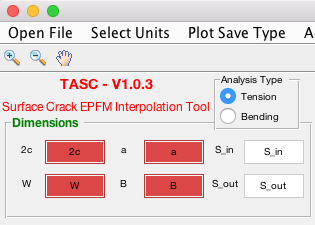
\includegraphics[width=0.6\columnwidth]{tasc-ui-changes}
\caption{\label{fig:tasc-ui-changes} Changes to TASC user interface to add support for bending models}
\end{figure}
Beyond user interface changes, other changes to TASC fall into one of two categories: adding support for test verification of interpolated bending models, and cleanup or simplification of existing code to remove deprecated functions or other code causing warnings with current releases of MATLAB.


\subsection{Adding Support for Bending Models}

TASC had incomplete support for bending models in the 1.0.2 release from 2014, and this support has been expanded to the level of validating models against experimental load-CMOD records. In addition to reading values from the \verb|S_in| and \verb|S_out| text entry boxes in the TASC user interface, steps to add this support include:
\begin{enumerate}
\item In \verb|interp_solution_fea_int.m| and \verb|plt_interp_details_CMOD_subplot_int.m|, checking for bending radio button state, and selecting the \verb|results| or the \verb|results_bending| variable from the database as necessary
\item \verb|interp_solution_fea_int.m|, checking for bending radio button state, and adjusting formulas for converting stress to reaction forces as necessary
\item In \verb|interp_solution_SCGui_CMOD_log_int.m| and \verb|interp_solution_fea_int.m|, checking for the \verb|moment_flag| attribute on a database result, and using the \verb|St_far| attribute for tension models or \verb|S_bend| attribute for bending models as needed
\end{enumerate}

\subsection{Cleanup, Simplification, and Fixing Deprecated Code}

Other changes made to the TASC source code include making indentation more consistent with MATLAB standards, removing unneeded punctuation, replacing deprecated function calls, and other items including:
\begin{enumerate}
\item In \verb|tasc.m|, added support for opening PDF help on MacOS,
\item In \verb|tasc.m|, disabling warnings for unused variables in function definitions generated by MATLAB's GUI development environment (GUIDE),
\item In \verb|tasc.m|, disabling warnings for unused callback functions generated by GUIDE,
\item In \verb|tasc.m|, replacing the deprecated \verb|strmatch| function with \verb|strcmp| for exact match comparison,
\item In \verb|EPFM_calcs_standalone.m|, making indentation consistent and replacing unused variables with placeholder variable \verb|~|,
\item In \verb|read_input_ntrp_file.m|, \verb|read_mat_props.m|, \verb|read_mat_props_interp.m|, and \\ \verb|read_testdata_sci.m|, replacing the deprecated \verb|strmatch| function with a new function \\ \verb|find_string_index| when searching for a substring.
\end{enumerate}
